%!TEX root = ../main.tex
\chapter{Il moto armonico}

\section{Cinematica del moto armonico}

Un moto armonico semplice è un moto la cui legge oraria è una funzione sinusoidale o cosinusoidale nel tempo. Si tratta di un andamento periodico, perché ad intervalli di tempo eguale il punto ripassa nella stessa posizione con la stessa velocità.

\begin{equation}
	\label{eqn:armonico}
	x(t)=A\cos(\omega_0 t+\Phi)
\end{equation}

\begin{figure}[htpb]
	\centering

	\tikzset{every picture/.style={line width=0.75pt}} %set default line width to 0.75pt        

	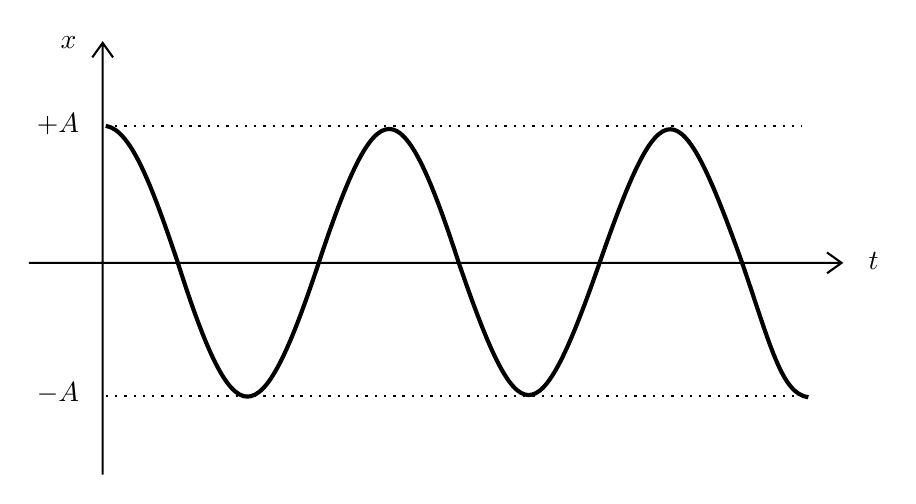
\begin{tikzpicture}[x=0.75pt,y=0.75pt,yscale=-1,xscale=1]
	%uncomment if require: \path (0,300); %set diagram left start at 0, and has height of 300

	% Plotting does not support converting to Tikz
	%Shape: Axis 2D [id:dp732307782075978] 
	\draw  (110,155) -- (501.5,155)(145.5,49) -- (145.5,257) (494.5,150) -- (501.5,155) -- (494.5,160) (140.5,56) -- (145.5,49) -- (150.5,56)  ;
	%Straight Lines [id:da7766397595927959] 
	\draw [line width=0.75]  [dash pattern={on 0.84pt off 2.51pt}]  (147,89) -- (482.5,89) ;
	%Straight Lines [id:da6094182586898851] 
	\draw [line width=0.75]  [dash pattern={on 0.84pt off 2.51pt}]  (147,219) -- (482.5,219) ;
	%Curve Lines [id:da2449173035027563] 
	\draw [line width=1.5]    (147,89) .. controls (159,90.75) and (169,117.25) .. (181.5,154.25) .. controls (209,240.75) and (221,241.25) .. (249.5,155.25) .. controls (278,69.25) and (289,68.75) .. (317,154.75) .. controls (346,239.25) and (355,240.75) .. (385,154.75) .. controls (415,68.75) and (423,69.75) .. (453.5,154.75) .. controls (467,193.75) and (472.5,218.25) .. (485.5,219.75) ;

	% Text Node
	\draw (124,88) node    {$+A$};
	% Text Node
	\draw (124,218) node    {$-A$};
	% Text Node
	\draw (517,154) node    {$t$};
	% Text Node
	\draw (129,49) node    {$x$};

	\end{tikzpicture}
\end{figure}

Il massimo spostamento dall'origine è $A$, che per questo prende il nome di ampiezza dell'oscillazione. Nell'argomento del coseno compare, oltre che a una funzione del tempo, un angolo che rappresenta la condizione iniziale del moto all'istante $t=0$ e per questo lo si chiama \textbf{fase iniziale}. Non è detto infatti che per $t=0$ la posizione del punto debba per forza coincidere con l'origine, ma potrebbe corrispondere ad un altro punto diverso da $0$. $\omega_0$ è il coefficiente di proporzionalità della variabile tempo e prende il nome di \textbf{pulsazione del moto}: è un parametro che rileva quanto sono rapide le oscillazioni.

Temporalmente il minimo intervallo di tempo tale per cui oltre ad esso il moto si ripete identico a se stesso (è infatti periodico),  è noto come \textbf{periodo}:

\[
	T \quad | \quad x(t)=x(t+T) \quad \forall t
\]

Possiamo calcolarlo come segue:

\begin{align*}
	x(t) &= x(t+T) \\
	A\cos(\omega_0 t+\Phi) &= A\cos(\omega_0 t +\omega_0 T+\Phi) \\
	\omega_0 t+\Phi &= \omega_0 t+\Phi+\omega_0 T \pm 2\pi \\
	T &= \frac{2\pi}{\omega_0}
\end{align*}

La pulsazione è dunque legata al periodo da questa relazione:

\[
	\boxed{\omega_0=\frac{2\pi}{T}}
\]

Si noti come il moto si ripeta velocemente quando la pulsazione è grande mentre è lento per bassi valori di essa. Infatti al crescere della pulsazione si accorcia il periodo e viceversa.

È comodo inoltre definire la \textbf{frequenza del moto}, ossia il numero di cicli, di periodi in un secondo. Più alta è la pulsazione, maggiore è la frequenza.

\[
	\boxed{f=\frac{1}{T}} \implies \boxed{\omega=2\pi f}
\]

Se si deriva la ~\eqref{eqn:armonico} una prima volta:

\[
	v(t)=\frac{dx}{dt}=-A\omega_0\sin(\omega_0 t+\Phi)
\]

\begin{figure}[htpb]
	\centering

	\tikzset{every picture/.style={line width=0.75pt}} %set default line width to 0.75pt        

	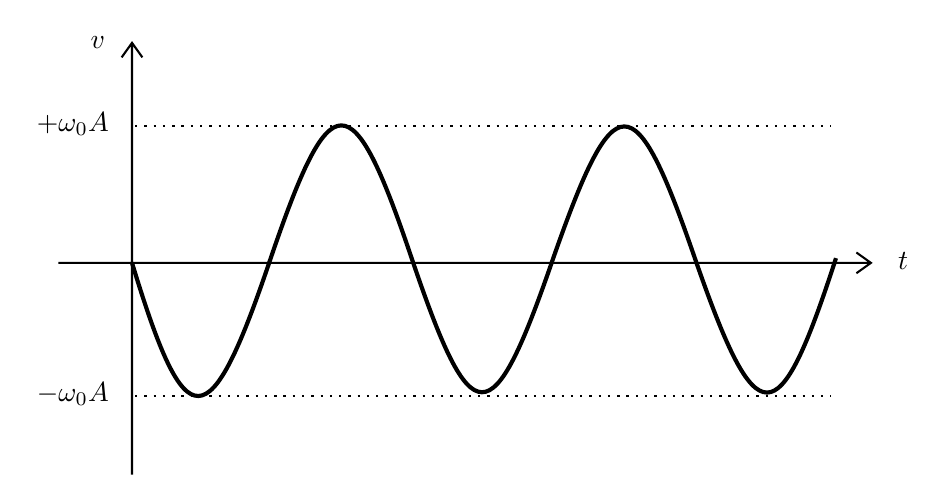
\begin{tikzpicture}[x=0.75pt,y=0.75pt,yscale=-1,xscale=1]
	%uncomment if require: \path (0,300); %set diagram left start at 0, and has height of 300

	% Plotting does not support converting to Tikz
	%Shape: Axis 2D [id:dp905263594609613] 
	\draw  (130,164.6) -- (521.5,164.6)(165.5,58.6) -- (165.5,266.6) (514.5,159.6) -- (521.5,164.6) -- (514.5,169.6) (160.5,65.6) -- (165.5,58.6) -- (170.5,65.6)  ;
	%Straight Lines [id:da3678422717394072] 
	\draw [line width=0.75]  [dash pattern={on 0.84pt off 2.51pt}]  (167,98.6) -- (502.5,98.6) ;
	%Straight Lines [id:da1458773151059063] 
	\draw [line width=0.75]  [dash pattern={on 0.84pt off 2.51pt}]  (167,228.6) -- (502.5,228.6) ;
	%Curve Lines [id:da5552577452439422] 
	\draw [line width=1.5]    (165.5,164.6) .. controls (191.5,250.25) and (202.5,250.75) .. (232.33,162.33) .. controls (261.33,77.33) and (271.33,76.67) .. (300.33,162.67) .. controls (329.33,248) and (338.67,248.67) .. (368.33,162.67) .. controls (398,78) and (407.33,77.33) .. (436.67,162.33) .. controls (466.67,248.67) and (476.67,248.67) .. (504.67,162.33) ;

	% Text Node
	\draw (137,97.6) node    {$+\omega _{0} A$};
	% Text Node
	\draw (137,227.6) node    {$-\omega _{0} A$};
	% Text Node
	\draw (537,163.6) node    {$t$};
	% Text Node
	\draw (149,58.6) node    {$v$};

	\end{tikzpicture}
\end{figure}

La velocità nel tempo varia con un seno dello stesso angolo e quindi oscillerà nel tempo con un periodo che è lo stesso ma con una funzione sfasata. L'oscillazione è compresa fra $A\omega_0$ e $-A\omega_0$. Analogamente si può calcolare l'accelerazione scalare come derivata della velocità nel tempo, ottenendo:

\[
	a(t)=\frac{dv}{dt}=-A\omega^2_0 t\cos(\omega_0 t+\Phi)
\]

L'accelerazione si annulla nel centro di oscillazione dove la velocità è massima e assume il valore massimo in modulo agli estremi, dove si inverte la velocità: inoltre essa è sempre proporzionale ed opposta allo spostamento dal centro di oscillazione. $a(t)$ e $x(t)$ sono una l'opposto dell'altra a parte una costante di proporzionalità. In particolare $a$ varia fra $\pm \omega^2_0 A$.
A parte il valore dell'ampiezza, le tre funzioni $x(t)$, $v(t)$ e $a(t)$ mostrano lo stesso andamento temporale: la forma e il periodo sono eguali, vi è solo uno spostamento di una rispetto all'altra lungo l'asse dei tempi. Quest'ultima caratteristica viene indicata dicendo che le funzioni sono sfasate fra loro.
In particolare la velocità è sfasata di $\frac{\pi}{2}$ rispetto allo spostamento (è in \emph{quadratura di fase}) mentre l'accelerazione è sfasata di $\pi$ sempre rispetto ad esso (è in \emph{opposizione di fase}). In pratica l'accelerazione è una oscillazione che avviene sempre come un seno ma il meno rappresenta tale sfasatura. Questa osservazione è ancora più interessante dal punto di vista analitico. Se infatti si ragiona su ciò, si nota che l'accelerazione è in relazione con $x(t)$ come segue:

\[
	a(t)=-A\omega^2_0 t\cos(\omega_0 t+\Phi)=-\omega^2_0\,x(t)
\]

Si ottiene quanto appena osservato: l'accelerazione è opposta a $x(t)$ a meno di una costante di proporzionalità.
Si può scrivere la relazione come equazione differenziale (relazione che lega cioè una funzione alle sue derivate):

\[
	\frac{d^2x}{dt^2}+\omega^2_0\,x(t)=0 \quad \forall t
\]

\begin{figure}[ht]
	\centering

	\tikzset{every picture/.style={line width=0.75pt}} %set default line width to 0.75pt        

	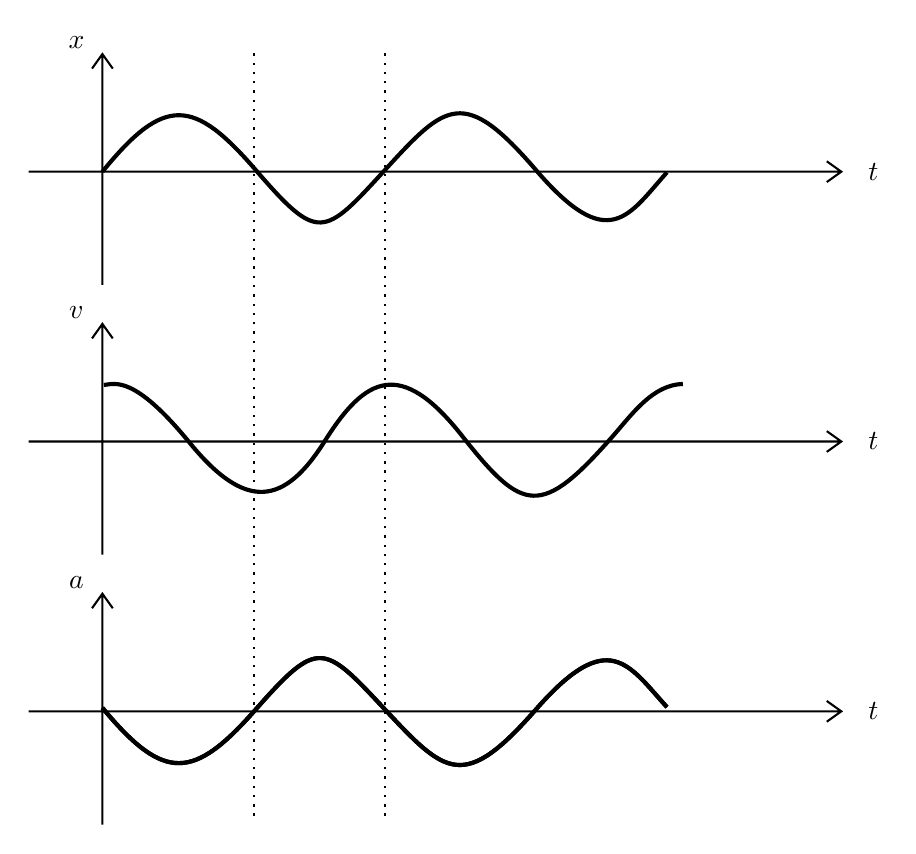
\begin{tikzpicture}[x=0.75pt,y=0.75pt,yscale=-1,xscale=1]
	%uncomment if require: \path (0,511); %set diagram left start at 0, and has height of 511

	%Shape: Axis 2D [id:dp07361889277532274] 
	\draw  (150,161.67) -- (541.5,161.67)(185.5,105) -- (185.5,216.2) (534.5,156.67) -- (541.5,161.67) -- (534.5,166.67) (180.5,112) -- (185.5,105) -- (190.5,112)  ;
	%Straight Lines [id:da48985214580087777] 
	\draw [line width=0.75]  [dash pattern={on 0.84pt off 2.51pt}]  (258.5,472) -- (258.5,103.6) ;
	% Plotting does not support converting to Tikz
	%Shape: Axis 2D [id:dp058897931948480364] 
	\draw  (150,291.67) -- (541.5,291.67)(185.5,235) -- (185.5,346.2) (534.5,286.67) -- (541.5,291.67) -- (534.5,296.67) (180.5,242) -- (185.5,235) -- (190.5,242)  ;
	%Shape: Axis 2D [id:dp6700287498310264] 
	\draw  (150,421.67) -- (541.5,421.67)(185.5,365) -- (185.5,476.2) (534.5,416.67) -- (541.5,421.67) -- (534.5,426.67) (180.5,372) -- (185.5,365) -- (190.5,372)  ;
	%Straight Lines [id:da5710725199192004] 
	\draw [line width=0.75]  [dash pattern={on 0.84pt off 2.51pt}]  (321.5,472) -- (321.5,103.6) ;
	%Curve Lines [id:da7575964396202544] 
	\draw [line width=1.5]    (185.5,161.67) .. controls (215.5,124.75) and (229.5,126.25) .. (259.5,161) .. controls (289.5,195.75) and (292,193.25) .. (321.5,161) .. controls (351,128.75) and (359.5,120.25) .. (394.5,161) .. controls (429.5,201.75) and (439,182.75) .. (457.5,162) ;
	%Curve Lines [id:da8424652798712617] 
	\draw [line width=1.5]    (185.5,419.97) .. controls (215.5,456.14) and (229.5,454.67) .. (259.5,420.62) .. controls (289.5,386.58) and (292,389.03) .. (321.5,420.62) .. controls (351,452.22) and (359.5,460.55) .. (394.5,420.62) .. controls (429.5,380.7) and (439,399.32) .. (457.5,419.64) ;
	%Curve Lines [id:da8424652798712617] 
	\draw [line width=1.5]    (185.5,419.97) .. controls (215.5,456.14) and (229.5,454.67) .. (259.5,420.62) .. controls (289.5,386.58) and (292,389.03) .. (321.5,420.62) .. controls (351,452.22) and (359.5,460.55) .. (394.5,420.62) .. controls (429.5,380.7) and (439,399.32) .. (457.5,419.64) ;
	%Curve Lines [id:da8976654485931836] 
	\draw [line width=1.5]    (186.17,264.42) .. controls (191.67,263.92) and (200.67,259.42) .. (227.67,292.42) .. controls (254.67,325.42) and (273.17,322.42) .. (292.67,291.42) .. controls (312.17,260.42) and (329.17,251.42) .. (358.67,288.79) .. controls (388.17,326.16) and (396.67,328.71) .. (431.67,288.79) .. controls (441.17,277.92) and (450.67,264.42) .. (465.17,263.92) ;

	% Text Node
	\draw (557,161.6) node    {$t$};
	% Text Node
	\draw (173,99.6) node    {$x$};
	% Text Node
	\draw (557,291.6) node    {$t$};
	% Text Node
	\draw (173,229.6) node    {$v$};
	% Text Node
	\draw (557,421.6) node    {$t$};
	% Text Node
	\draw (173,359.6) node    {$a$};

	\end{tikzpicture}
	%\caption{Andamento di spazio, velocità e accelerazione in un moto armonico}
    %\label{fig:equazioniMotoArmoicoDerivate}
\end{figure}

Essa è detta \textbf{equazione differenziale caratteristica del moto armonico}. Un moto armonico è dunque un moto che soddisfa tale relazione. Le funzioni seno e coseno e le loro combinazioni lineari, sono tutte e sole le funzioni che soddisfano a questa condizione nel campo reale.

Quest'ultimo fatto porta a osservare esplicitamente che le proprietà generali del moto armonico semplice restano eguali se invece della funzione ~\eqref{eqn:armonico} si fosse utilizzata la funzione coseno. Le due funzioni infatti differiscono solo per un termine di sfasamento pari a $\frac{\pi}{2}$.

\section{Esempi di moti armonici semplici}

\subsection{Forza elastica}

Si consideri il caso di un corpo di massa $m$ appoggiato a un piano orizzontale perfettamente liscio, vincolato a una molla di costante elastica $k$. Inizialmente il sistema si trova in una condizione di riposo. Si definisce un asse $x$ in cui l'origine corrisponde alla posizione in cui si trova il corpo a riposo. La molla viene allungata di uno spostamento $x$, così che il corpo trasli in avanti. L'obbiettivo è di ricavare la legge oraria a cui esso sarà soggetto. Dal punto di vista dinamico, in direzione verticale agisce la forza peso perfettamente bilanciata dalla reazione normale. In direzione orizzontale vi è la forza di richiamo della molla.

Quando il corpo ritorna nella posizione di equilibrio, esso non si ferma perché ha acquisito velocità, ma continua a deformare la molla che lo richiama indietro. Il moto sarà un'oscillazione perpetua: un moto armonico.

\[
	x: \qquad -kx=ma
\]

Ricordando che $x$ non sarà costante nel tempo:

\[
	-kx=m\frac{d^2x}{dx^2} \implies \frac{d^2x}{dt^2}+\frac{k}{m}x=0
\]

Si trova che il sistema meccanico dato dal corpo attaccato alla molla reagisce alla perturbazione dell'equilibrio con una accelerazione di richiamo proporzionale allo spostamento subito: si tratta di un moto armonico. Dato che in esso il coefficiente di proporzionalità è l'opposto del quadrato della pulsazione, nel caso di una molla si trova:

\[
	\frac{d^2x}{dt^2}+\omega^2_0 x=0 \implies \omega_0=\sqrt{\frac{k}{m}}
\]

L'asse $x$ del primo grafico nella figura vista prima rappresenta la posizione nel tempo, è come se si potesse disegnare a lato la molla. Quando passa nella posizione di riposo il corpo è stato accelerato per aumentare la sua velocità che è diventata massima. Quindi il corpo va avanti fino a che la molla non si comprime.  Nei punti di massima compressione o massimo allungamento l'accelerazione è massima o minima e la velocità è nulla (il corpo si ferma) mentre nel punto di equilibrio non vi è accelerazione ma una velocità che è massima.

Abbiamo visto un esempio di moto armonico dato da una forza in direzione tangente al moto, in cui essa modifica il valore della velocità. Vediamo ora un esempio con una \textbf{forza centripeta}, ossia che fa variare la direzione della velocità.

\subsection{Il pendolo semplice}

Il pendolo semplice è costituito da un punto materiale appeso tramite una fune inestensibile e di massa trascurabile. La situazione di equilibrio statico è quella per cui il filo è sospeso lungo la verticale. La forza esercitata da esso è $\vec{T}=m\vec{g}$. Se si sposta il punto dalla verticale, ossia se viene data al filo una certa inclinazione che si indica con l'angolo $\vartheta$, esso inizia ad oscillare attorno alla posizione di equilibrio, lungo un arco di circonferenza di raggio $L$. Il corpo in assenza di attriti continua a oscillare e quello che si ottiene è anche in questo caso un moto armonico semplice.

\begin{figure}[htpb]
	\centering

	% Pattern Info
	 
	\tikzset{
	pattern size/.store in=\mcSize, 
	pattern size = 5pt,
	pattern thickness/.store in=\mcThickness, 
	pattern thickness = 0.3pt,
	pattern radius/.store in=\mcRadius, 
	pattern radius = 1pt}
	\makeatletter
	\pgfutil@ifundefined{pgf@pattern@name@_spdknvuu7}{
	\pgfdeclarepatternformonly[\mcThickness,\mcSize]{_spdknvuu7}
	{\pgfqpoint{0pt}{0pt}}
	{\pgfpoint{\mcSize+\mcThickness}{\mcSize+\mcThickness}}
	{\pgfpoint{\mcSize}{\mcSize}}
	{
	\pgfsetcolor{\tikz@pattern@color}
	\pgfsetlinewidth{\mcThickness}
	\pgfpathmoveto{\pgfqpoint{0pt}{0pt}}
	\pgfpathlineto{\pgfpoint{\mcSize+\mcThickness}{\mcSize+\mcThickness}}
	\pgfusepath{stroke}
	}}
	\makeatother
	\tikzset{every picture/.style={line width=0.75pt}} %set default line width to 0.75pt        

	\begin{tikzpicture}[x=0.75pt,y=0.75pt,yscale=-1,xscale=1]
	%uncomment if require: \path (0,351); %set diagram left start at 0, and has height of 351

	%Shape: Rectangle [id:dp19908194141643554] 
	\draw  [draw opacity=0][pattern=_spdknvuu7,pattern size=6pt,pattern thickness=0.75pt,pattern radius=0pt, pattern color={rgb, 255:red, 222; green, 222; blue, 222}] (80,41.5) -- (492.5,41.5) -- (492.5,69) -- (80,69) -- cycle ;
	%Straight Lines [id:da8854451216886683] 
	\draw    (80,69) -- (492.5,69) ;
	%Shape: Arc [id:dp8757101389668807] 
	\draw  [draw opacity=0][dash pattern={on 0.84pt off 2.51pt}] (383.26,168.27) .. controls (349.7,222.48) and (289.69,258.59) .. (221.25,258.59) .. controls (171.41,258.59) and (126.03,239.44) .. (92.09,208.09) -- (221.25,68.17) -- cycle ; \draw  [dash pattern={on 0.84pt off 2.51pt}] (383.26,168.27) .. controls (349.7,222.48) and (289.69,258.59) .. (221.25,258.59) .. controls (171.41,258.59) and (126.03,239.44) .. (92.09,208.09) ;
	%Shape: Circle [id:dp9647791556970287] 
	\draw  [fill={rgb, 255:red, 0; green, 0; blue, 0 }  ,fill opacity=1 ] (218,69) .. controls (218,67.21) and (219.46,65.75) .. (221.25,65.75) .. controls (223.04,65.75) and (224.5,67.21) .. (224.5,69) .. controls (224.5,70.79) and (223.04,72.25) .. (221.25,72.25) .. controls (219.46,72.25) and (218,70.79) .. (218,69) -- cycle ;
	%Straight Lines [id:da02623529304163541] 
	\draw  [dash pattern={on 0.84pt off 2.51pt}]  (221.25,68.17) -- (221.25,258.31) ;
	%Straight Lines [id:da43326551309148487] 
	\draw    (221.25,68.17) -- (328.9,223.64) ;
	%Shape: Ellipse [id:dp9763602525450497] 
	\draw  [draw opacity=0][fill={rgb, 255:red, 155; green, 155; blue, 155 }  ,fill opacity=1 ] (315.7,223.64) .. controls (315.7,216.35) and (321.61,210.44) .. (328.9,210.44) .. controls (336.19,210.44) and (342.1,216.35) .. (342.1,223.64) .. controls (342.1,230.93) and (336.19,236.83) .. (328.9,236.83) .. controls (321.61,236.83) and (315.7,230.93) .. (315.7,223.64) -- cycle ;
	%Straight Lines [id:da3604521273003396] 
	\draw [line width=1.5]    (328.9,223.64) -- (328.9,314.75) ;
	\draw [shift={(328.9,318.75)}, rotate = 270] [fill={rgb, 255:red, 0; green, 0; blue, 0 }  ][line width=0.08]  [draw opacity=0] (13.4,-6.43) -- (0,0) -- (13.4,6.44) -- (8.9,0) -- cycle    ;
	%Straight Lines [id:da16498016296525497] 
	\draw [line width=1.5]    (331.14,221.4) -- (283.26,151.81) ;
	\draw [shift={(280.99,148.51)}, rotate = 415.47] [fill={rgb, 255:red, 0; green, 0; blue, 0 }  ][line width=0.08]  [draw opacity=0] (13.4,-6.43) -- (0,0) -- (13.4,6.44) -- (8.9,0) -- cycle    ;
	%Straight Lines [id:da0071920943467709275] 
	\draw [line width=1.5]    (328.9,223.64) -- (249.7,108.19) ;
	\draw [shift={(247.44,104.89)}, rotate = 415.55] [fill={rgb, 255:red, 0; green, 0; blue, 0 }  ][line width=0.08]  [draw opacity=0] (13.4,-6.43) -- (0,0) -- (13.4,6.44) -- (8.9,0) -- cycle    ;
	%Shape: Arc [id:dp8965644261235546] 
	\draw  [draw opacity=0] (263.41,128.79) .. controls (251.46,137.12) and (236.92,142) .. (221.25,142) .. controls (220.96,142) and (220.67,142) .. (220.37,141.99) -- (221.25,68.17) -- cycle ; \draw   (263.41,128.79) .. controls (251.46,137.12) and (236.92,142) .. (221.25,142) .. controls (220.96,142) and (220.67,142) .. (220.37,141.99) ;
	%Straight Lines [id:da40890744138766677] 
	\draw    (210.07,70.41) -- (210.07,256.07) ;
	\draw [shift={(210.07,256.07)}, rotate = 270] [color={rgb, 255:red, 0; green, 0; blue, 0 }  ][line width=0.75]    (0,5.59) -- (0,-5.59)   ;
	\draw [shift={(210.07,70.41)}, rotate = 270] [color={rgb, 255:red, 0; green, 0; blue, 0 }  ][line width=0.75]    (0,5.59) -- (0,-5.59)   ;
	%Straight Lines [id:da01871836867451715] 
	\draw [line width=1.5]    (328.9,223.64) -- (287.11,250.95) ;
	\draw [shift={(283.76,253.14)}, rotate = 326.83000000000004] [fill={rgb, 255:red, 0; green, 0; blue, 0 }  ][line width=0.08]  [draw opacity=0] (13.4,-6.43) -- (0,0) -- (13.4,6.44) -- (8.9,0) -- cycle    ;
	%Straight Lines [id:da07884360167382432] 
	\draw    (328.9,223.64) -- (397.85,323.22) ;
	%Straight Lines [id:da4270548204578508] 
	\draw [line width=1.5]    (383.64,140.9) -- (355.87,100.55) ;
	\draw [shift={(353.61,97.25)}, rotate = 415.47] [fill={rgb, 255:red, 0; green, 0; blue, 0 }  ][line width=0.08]  [draw opacity=0] (13.4,-6.43) -- (0,0) -- (13.4,6.44) -- (8.9,0) -- cycle    ;
	%Straight Lines [id:da3070934302985917] 
	\draw [line width=1.5]    (383.64,140.9) -- (423.99,113.14) ;
	\draw [shift={(427.29,110.87)}, rotate = 505.47] [fill={rgb, 255:red, 0; green, 0; blue, 0 }  ][line width=0.08]  [draw opacity=0] (13.4,-6.43) -- (0,0) -- (13.4,6.44) -- (8.9,0) -- cycle    ;
	%Straight Lines [id:da8303876221439561] 
	\draw [line width=0.75]  [dash pattern={on 0.84pt off 2.51pt}]  (374.04,289.25) -- (328.9,318.75) ;
	%Straight Lines [id:da8777416855485225] 
	\draw [line width=1.5]    (371.77,285.95) -- (328.9,223.64) ;
	\draw [shift={(374.04,289.25)}, rotate = 235.47] [fill={rgb, 255:red, 0; green, 0; blue, 0 }  ][line width=0.08]  [draw opacity=0] (13.4,-6.43) -- (0,0) -- (13.4,6.44) -- (8.9,0) -- cycle    ;
	%Straight Lines [id:da1372972802325747] 
	\draw [line width=0.75]  [dash pattern={on 0.84pt off 2.51pt}]  (328.9,318.75) -- (283.76,253.14) ;
	%Shape: Arc [id:dp43221342740275226] 
	\draw  [draw opacity=0] (346.1,248.36) .. controls (341.22,251.76) and (335.29,253.75) .. (328.9,253.75) .. controls (328.78,253.75) and (328.66,253.75) .. (328.54,253.75) -- (328.9,223.64) -- cycle ; \draw   (346.1,248.36) .. controls (341.22,251.76) and (335.29,253.75) .. (328.9,253.75) .. controls (328.78,253.75) and (328.66,253.75) .. (328.54,253.75) ;

	% Text Node
	\draw (272.79,102.1) node    {$\vec{T}$};
	% Text Node
	\draw (307.84,148.33) node    {$\vec{R}_{n}$};
	% Text Node
	\draw (276.78,265.3) node    {$\vec{R}_{t}$};
	% Text Node
	\draw (328.79,328.76) node    {$m\vec{g}$};
	% Text Node
	\draw (352.27,223.56) node    {$P$};
	% Text Node
	\draw (248.44,148.97) node    {$\vartheta $};
	% Text Node
	\draw (332.95,197.12) node    {$m$};
	% Text Node
	\draw (201.21,159.14) node    {$L$};
	% Text Node
	\draw (442.29,108.1) node    {$\vec{u}_{t}$};
	% Text Node
	\draw (340.79,96.6) node    {$\vec{u}_{n}$};
	% Text Node
	\draw (339.44,261.47) node    {$\vartheta $};

	\end{tikzpicture}
\end{figure}

Per calcolare la legge oraria, conviene descrivere la posizione del punto in termini di posizione angolare. Il nostro obbiettivo è ricavare $\vartheta (t)$, con verso positivo quando va in verso antiorario. Andiamo a utilizzare la seconda legge della dinamica. Le forze agenti su punto $P$ sono il peso $m\vec{g}$ e la tensione del filo $T$, per cui il moto è regolato da $m\vec{g}+\vec{T}=m\vec{a}$. Conviene scomporre la seconda legge della dinamica in direzione tangente e normale alla traiettoria. Si prende la direzione tangente concorde al verso positivo dell'angolo, mentre la direzione normale sarà diretta verso l'interno della concavità.

\[
	\begin{cases} \vec{u}_t: \quad -mg\sin\vartheta=ma_t \\ \vec{u}_n: \quad T-mg\cos\vartheta=ma_n \end{cases}
\]

Il segno negativo della componente lungo la traiettoria è dovuto solo fatto che la forza ha segno opposto rispetto a quello della coordinata $s$ sulla traiettoria. Fisicamente $R_t=-mg\sin\vartheta$ è una forza di richiamo che tende a riportare il punto sulla verticale, anche se non è di direzione costante come nel caso delle forze elastiche.

\[
	-g\sin\vartheta=\frac{dv}{dt}=\frac{d\omega L}{dt}=\frac{d\omega}{dt}\,L=L\frac{d^2\vartheta}{dt^2}
\]

L'accelerazione normale sarà $\frac{v^2}{L}$. Si usa la legge al di sopra perché informa su come varia nel tempo la velocità scalare, la scomposizione tangente è sempre quella che informa sulla legge oraria.

\[
	-g\frac{\sin\vartheta}{L}=\frac{d^2\vartheta}{dt^2}
\]

Si è trovata una relazione che lega la posizione angolare alla derivata seconda. La soluzione non è esattamente quella del moto armonico ma, per valori molto piccoli dell'angolo, si può attuare l'approssimazione:

\[
	\sin\vartheta=\vartheta+\frac{\vartheta^3}{3!}+\dots \implies \sin\vartheta \simeq \vartheta \implies -\frac{g}{L}\vartheta(t)=\frac{d^2\vartheta}{dt^2}
\]

Per $\vartheta \le 0.122 \,\text{rad}, \,\sin\vartheta$ può essere approssimato a $\vartheta$ commettendo un errore relativo che è sempre minore di $10^{-3}$. Si ha allora:

\begin{equation}
	\frac{d^2\vartheta}{dt^2}+\frac{g}{L}\vartheta(t)=0
\end{equation}

Si trova così l'equazione differenziale per piccole oscillazioni. In conclusione il moto del pendolo è oscillatorio armonico quando l'ampiezza delle oscillazioni è piccola. La legge oraria del moto è:

\[
	\vartheta(t)=\vartheta_0\cos(\omega t+\Phi)
\]

Si può affermare che il pendolo si muove di moto armonico con pulsazione caratteristica pari a:

\[
	\omega=\sqrt{\frac{g}{L}}
\]

Si nota che il periodo del pendolo non dipende dalla massa ma dall'accelerazione di gravità e dalla lunghezza del filo. Inoltre esso non dipende nemmeno dall'ampiezza (isocronismo delle piccole oscillazioni).
Se si vuole ottenere la legge oraria dello spostamento lungo l'arco di circonferenza si sfrutta la relazione:

\[
	s(t)=L\,\vartheta(t)=L\vartheta_0\cos(\omega t+\Phi)
\]

Lo studio del moto del pendolo è interessante perché mostra un moto armonico che non avviene su una traiettoria rettilinea, permettendo di osservare che la legge oraria si ottiene concentrandosi sulle componenti tangenti delle forza, proprio perché sono quelle che modificano il valore della velocità. Tali forze tangenti si chiamano anche forze vive. L'altra scomposizione della seconda legge della dinamica in direzione normale alla traiettoria dà una informazione sulle forze che permettono al punto materiale di riuscire a mantenere una traiettoria curvilinea. La tensione di una fune è un esempio tipico di una forza che permette a un corpo di curvare. Essa non si mantiene costante nel tempo ma cambia valore al variare della posizione. Perché il filo non si rompa la tensione deve essere minore di $T_{MAX}$. La velocità in un moto armonico è minima agli estremi, dove il moto si inverte, ed è massima sulla verticale, in questo punto anche la forza peso è massima. Quindi il punto critico in termini di tensione massima è quest'ultimo.
Il moto del pendolo semplice può avvenire con velocità iniziale nulla purché l'angolo sia diverso da zero. Quando l'ampiezza delle oscillazioni non è piccola il moto è ancora periodico, ma non armonico, e il periodo dipende dall'ampiezza.

\section{Studio energetico di un moto armonico}

Dal punto di vista energetico, un corpo che si muove sottoposto alla forza elastica, conservativa, avrà un energia meccanica costante perché forza peso e reazione normale non compiono lavoro.

Quando la molla raggiunge il punto di massima compressione l'energia cinetica si annulla. Essa diventa poi massima quando il corpo ripassa per la posizione di riposo e via dicendo.
L'ampiezza vale: $A^2\omega_0^2$.

\[
	E_k=\frac{1}{2}mv^2(t)=\frac{1}{2}mA^2\omega_0^2\sin^2(\omega_0 t+\Phi)
\]

C'è un continuo scambio di contributo energetico fra energia cinetica e energia potenziale. Dimostriamolo analiticamente:

\begin{gather*}
	E_{\text{pot}}=\frac{1}{2}kx^2(t)=\frac{1}{2}kA^2\cos^2(\omega_0 t+\Phi) \\
	E_{\text{mecc}}=\frac{1}{2}kA^2\cos^2(\omega_0 t+\Phi)+\frac{1}{2}mA^2\omega_0^2\sin^2(\omega_0 t+\Phi)
\end{gather*}

attuando la sostituzione $\omega_0=\sqrt{\frac{k}{m}}$ si ha:

\[
	E_{\text{mecc}}=\frac{1}{2}kA^2\cos^2(\omega_0 t+\Phi)+\frac{1}{2}kA^2\\sin^2(\omega_0 t+\Phi)=\frac{1}{2}kA^2
\]

Sebbene i contributi energetici oscillino nel tempo si nota che l'energia meccanica è sempre costante.

\begin{figure}[htpb]
	\centering

	\tikzset{every picture/.style={line width=0.75pt}} %set default line width to 0.75pt        

	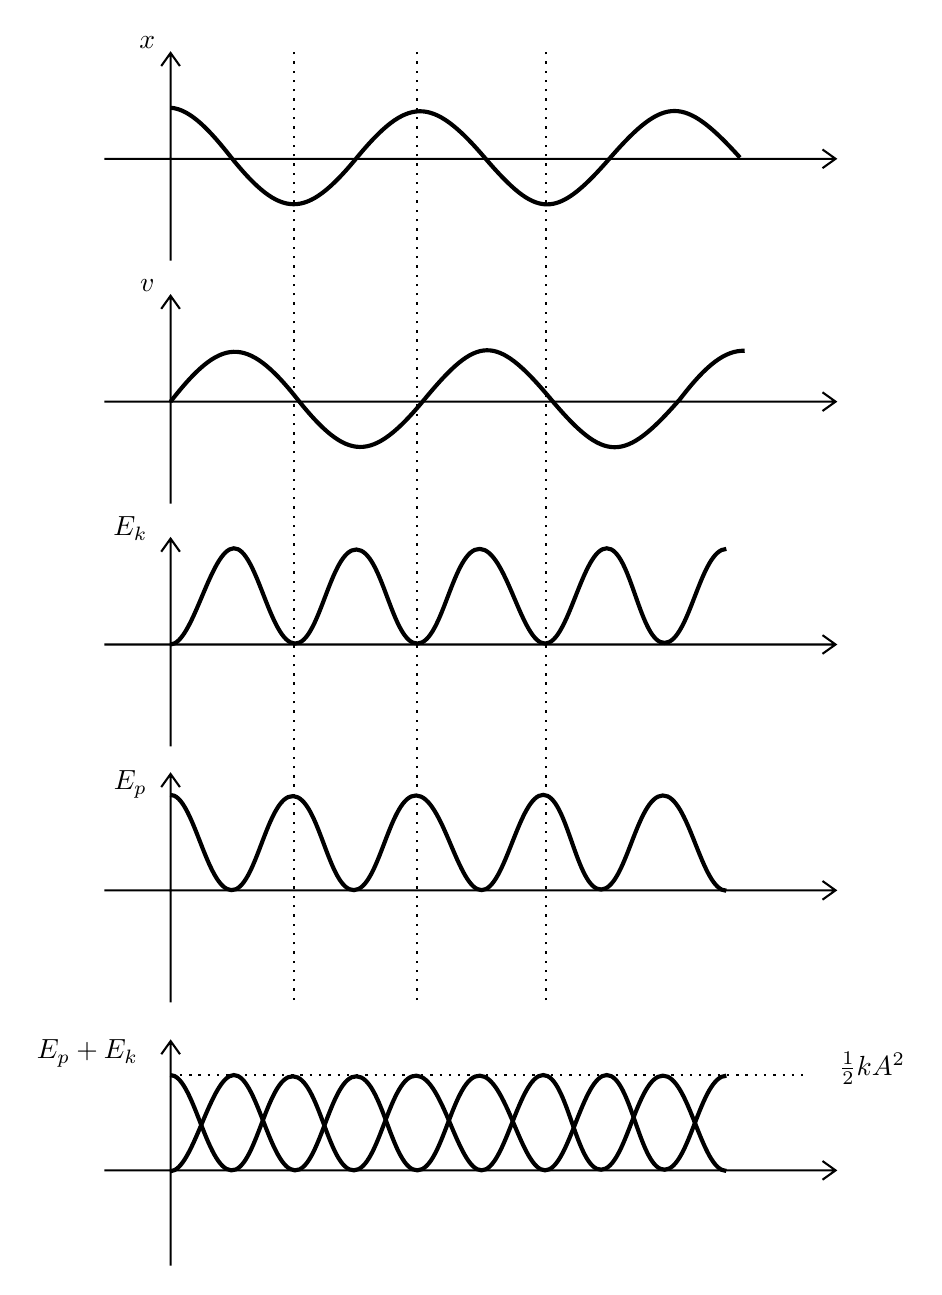
\begin{tikzpicture}[x=0.75pt,y=0.75pt,yscale=-0.9,xscale=0.9]
	%uncomment if require: \path (0,822); %set diagram left start at 0, and has height of 822

	% Plotting does not support converting to Tikz
	%Shape: Axis 2D [id:dp9554882578986952] 
	\draw  (79,181.67) -- (470.5,181.67)(114.5,125) -- (114.5,236.2) (463.5,176.67) -- (470.5,181.67) -- (463.5,186.67) (109.5,132) -- (114.5,125) -- (119.5,132)  ;
	%Straight Lines [id:da5272545840794085] 
	\draw [line width=0.75]  [dash pattern={on 0.84pt off 2.51pt}]  (180.5,632) -- (180.5,123.6) ;
	%Shape: Axis 2D [id:dp3531664678382227] 
	\draw  (79,311.67) -- (470.5,311.67)(114.5,255) -- (114.5,366.2) (463.5,306.67) -- (470.5,311.67) -- (463.5,316.67) (109.5,262) -- (114.5,255) -- (119.5,262)  ;
	% Plotting does not support converting to Tikz
	%Shape: Axis 2D [id:dp6720567158093034] 
	\draw  (79,441.67) -- (470.5,441.67)(114.5,385) -- (114.5,496.2) (463.5,436.67) -- (470.5,441.67) -- (463.5,446.67) (109.5,392) -- (114.5,385) -- (119.5,392)  ;
	%Straight Lines [id:da8589279622426254] 
	\draw [line width=0.75]  [dash pattern={on 0.84pt off 2.51pt}]  (246.5,632) -- (246.5,123.6) ;
	%Straight Lines [id:da9613052196013632] 
	\draw [line width=0.75]  [dash pattern={on 0.84pt off 2.51pt}]  (315.5,632) -- (315.5,123.6) ;
	% Plotting does not support converting to Tikz
	%Shape: Axis 2D [id:dp7437622625843014] 
	\draw  (79,573.28) -- (470.5,573.28)(114.5,511) -- (114.5,633.2) (463.5,568.28) -- (470.5,573.28) -- (463.5,578.28) (109.5,518) -- (114.5,511) -- (119.5,518)  ;
	%Shape: Axis 2D [id:dp029865456838393145] 
	\draw  (79,723.2) -- (470.5,723.2)(114.55,654) -- (114.55,774.2) (463.5,718.2) -- (470.5,723.2) -- (463.5,728.2) (109.55,661) -- (114.55,654) -- (119.55,661)  ;
	%Straight Lines [id:da6865054473899408] 
	\draw [line width=0.75]  [dash pattern={on 0.84pt off 2.51pt}]  (114.55,672.2) -- (456.55,672.2) ;
	%Curve Lines [id:da186605963203905] 
	\draw [line width=1.5]    (114.33,154.33) .. controls (125.25,154.88) and (136.25,167.38) .. (147,181) .. controls (173.75,214.13) and (186.75,214.38) .. (214,181.33) .. controls (241.25,148.29) and (254,147.63) .. (282.33,180.67) .. controls (310.67,213.71) and (320.25,215.13) .. (349.67,181.33) .. controls (379.08,147.54) and (389.25,147.88) .. (419.33,181) ;
	%Curve Lines [id:da29313157364483367] 
	\draw [line width=1.5]    (114.5,311.67) .. controls (141.25,277.28) and (154.75,275.54) .. (182,309.85) .. controls (209.25,344.15) and (222,344.84) .. (250.33,310.54) .. controls (278.67,276.23) and (288.25,274.76) .. (317.67,309.85) .. controls (347.08,344.93) and (357.25,344.58) .. (387.33,310.19) .. controls (401.57,291.57) and (411.57,284.14) .. (421.86,284.43) ;
	%Curve Lines [id:da2916033657930399] 
	\draw [line width=1.5]    (114.5,441.67) .. controls (126.67,441.17) and (136,390.5) .. (148.33,390.17) .. controls (160.67,389.83) and (167.67,440.5) .. (181,441.17) .. controls (194.33,441.83) and (200,390.5) .. (214,390.83) .. controls (228,391.17) and (233,441.5) .. (246.67,441.17) .. controls (260.33,440.83) and (265.67,390.17) .. (280,390.5) .. controls (294.33,390.83) and (302.33,441.17) .. (315,441.17) .. controls (327.67,441.17) and (335,390.17) .. (348,390.17) .. controls (361,390.17) and (365.67,441.17) .. (379,440.83) .. controls (392.33,440.5) and (398,390.83) .. (412,390.5) ;
	%Curve Lines [id:da7476925369183249] 
	\draw [line width=1.5]    (114.33,522.17) .. controls (126.67,521.83) and (133.67,572.5) .. (147,573.17) .. controls (160.33,573.83) and (166,522.5) .. (180,522.83) .. controls (194,523.17) and (199,573.5) .. (212.67,573.17) .. controls (226.33,572.83) and (231.67,522.17) .. (246,522.5) .. controls (260.33,522.83) and (268.33,573.17) .. (281,573.17) .. controls (293.67,573.17) and (301,522.17) .. (314,522.17) .. controls (327,522.17) and (331.67,573.17) .. (345,572.83) .. controls (358.33,572.5) and (364,522.83) .. (378,522.5) .. controls (392,522.17) and (398.67,573.5) .. (412,573.5) ;
	%Curve Lines [id:da22569658489583788] 
	\draw [line width=1.5]    (114.33,672.17) .. controls (126.67,671.83) and (133.67,722.5) .. (147,723.17) .. controls (160.33,723.83) and (166,672.5) .. (180,672.83) .. controls (194,673.17) and (199,723.5) .. (212.67,723.17) .. controls (226.33,722.83) and (231.67,672.17) .. (246,672.5) .. controls (260.33,672.83) and (268.33,723.17) .. (281,723.17) .. controls (293.67,723.17) and (301,672.17) .. (314,672.17) .. controls (327,672.17) and (331.67,723.17) .. (345,722.83) .. controls (358.33,722.5) and (364,672.83) .. (378,672.5) .. controls (392,672.17) and (398.67,723.5) .. (412,723.5) ;
	%Curve Lines [id:da7782549887315116] 
	\draw [line width=1.5]    (114.5,723.67) .. controls (126.67,723.17) and (136,672.5) .. (148.33,672.17) .. controls (160.67,671.83) and (167.67,722.5) .. (181,723.17) .. controls (194.33,723.83) and (200,672.5) .. (214,672.83) .. controls (228,673.17) and (233,723.5) .. (246.67,723.17) .. controls (260.33,722.83) and (265.67,672.17) .. (280,672.5) .. controls (294.33,672.83) and (302.33,723.17) .. (315,723.17) .. controls (327.67,723.17) and (335,672.17) .. (348,672.17) .. controls (361,672.17) and (365.67,723.17) .. (379,722.83) .. controls (392.33,722.5) and (398,672.83) .. (412,672.5) ;

	% Text Node
	\draw (102,119.6) node    {$x$};
	% Text Node
	\draw (102,249.6) node    {$v$};
	% Text Node
	\draw (93,379.6) node    {$E_{k}$};
	% Text Node
	\draw (93,516.6) node    {$E_{p}$};
	% Text Node
	\draw (70,660.6) node    {$E_{p} +E_{k}$};
	% Text Node
	\draw (490,668.6) node    {$\frac{1}{2} kA^{2}$};

	\end{tikzpicture}
\end{figure}
